\externaldocument{4/chapter4.tex}
\section{Systems Dynamics}
\label{sec:sysdyn}
As the understanding of biology has grown, so too do the means and methods by which this new knowledge is attained. The various levels of life can be represented in a hierarchy, such as organelles, cell and tissues up through organisms, community and species. Inter- or intra- relationships between subgroup members can utilize analytical techniques from other disciplines and need not be reinvented. An interdisciplinary approach to biological systems has borrowed many tools from the domains of mathematics and physics. Complex systems science studies the \textbf{emergence} of organizational structure leading to function which cannot be explained by investigating individual constituent components alone. A systems approach is needed to track the many the collective, macroscopic effects individual interacting components spontaneously birth. Derived from the latin \emph{plexus} meaning intertwined, the ying to complexity\'s yang is separability. Reducing complex systems to components removes novel information regarding interaction and thus limits predictive capabilities on that same system. This is a major motivation for inferring the network using ODEs at once rather than many MI methods which infer links individually in relation to one another, discussed in \cref{sec:models} on page~\pageref{sec:models}.

The following offers a brief introduction to those relevant attributes based upon the premise that characteristics/properties, among other things, can be a strong indicator of ability to correctly, accurately and reproducibly infer networks. Our group has been specifically focused on three such characteristics, namely sparsity, the signal-to-noise ratio, and condition number or Interampatteness discussed in \cref{sec:biosys} on page~\pageref{sec:biosys}.


\subsection{Two Distinct, General Aims}
\label{sec:purpose}
Gardner (2005) offers two types of networks based on two distinct aims. The first offers a \textbf{mechanistic} view of direct, physical interactions among biomolecules via chemical bonding. To leave a single biomolecule unquantified risks its activity being interpreted as that of another molecule, and thus this method is both highly expansive as well as rather dubious to characterize. Thus, a second \textbf{influential} approach is proposed, whereby indirect interactions are allowed by the added caveat that any measured interaction is necessarily not-direct. This type of network contains interactions capable of passing through innumerable intermediate biomolecules and indeed levels of biology on its way to affecting its eventual target.

A major assumption of this research lies in the nature of the response to perturbation, \ie that the system has reached some state whereupon interaction between genes is stable and major change is less likely. This surely simplifies reality but is quite powerful for modeling the large, unchanging tendencies driving operations crucial to cellular life, and as such has seen extensive use in the field of systems biology. Work has also been done to show that nonlinear systems can be approximated fairly well using linear models when the system is in steady state \citep{wildenhain2006reconstructing}. These build to the main points of \cref{sec:practical}

% \subsection{Time-Series}
% \label{time}
% % Time-Series

% Non-linear time series/ Michaelis-Menten/ hill kinetics Time
% LDS/ Linear

\subsection{Regulation is as much about \emph{what} as it is \emph{when}}
\label{sec:regwhatwhen}
Dynamics is in its most basic form a study of what and when -- by how much has any given system element changed over any given element of time. Determining these rates of change is the primary concern of experimental biologist wishing to better understand their investigative niche, for example. They bind many such studied factors together into a system using equations defining their rates of change in relation to one another using a \textbf{system of equations}. As with all models, the simpler the equations, \ie the fewer parameters and lower the complexity, the fewer degrees of freedom which calls for less data than the complex alternative. However the description of the given system can vary in appreciable ways: where \textbf{linear} relationships enable simplification at the cost of reflecting abstractions of truth, \textbf{nonlinearity} presents the potential for higher resolution, but risks misrepresenting underlying biology in its own right. Nonlinear models might be especially useful for modeling the robust capabilities of many natural systems, for example the adaptive ability of some bacterial species to maintain similar function and activity while changing uptake among several fundamentally different growth medium, \ie modeling diauxic growth of E.coli on glucose and lactose \citep{wong1997mathematical}. In this case it would be enough to have a linear model simply not distinguish between media, and simply account for continued growth over time after a lag period in which the bacterium adjusted to the new environment.


\subsection{Parameter Estimation}
\label{sec:parest}
A systems encompasses a means of mapping two sets of variables to one another. Convention dictates this function use various assemblies of parameters to equate independent and dependent variables. Thus we seek to use a known linear model to determine the parameter values which will fit observed data to model outputs. Here our investigation is focused on changes in concentrations over time, and thus an element of time must be incorporated, making our models dynamic via implementation as \textbf{first-order} (those relying on function's first derivative) \textbf{linear differential equations}. Also, because the measurements we gather are prone to error compounded by the non-static quantity we strive to characterize, elements of noise persist into our data, and so an estimation of noise is added. As a linear model we can describe this system as follows:

\begin{equation}
\label{eq:Linearmap}
  \mY = -\mA^{-1}(\mP+\mF)+ \mE,
\end{equation}
% \myequations{Linear Map}

where the independent measurements Y map to the known experimental design P to solve for a network structure, A, which explains both while also accounting for systematic error, E. Since we are solving for the parameters that facilitate the mapping of variables to one another, this case is known as an inverse problem. Many methods can solve this equation, but an optimal minimum-variance, unbiased estimator (MVUE) for sufficiently large datasets remains largely elusive \citep{kay1993fundamentals}. 



\subsection{Regression}
\label{sec:regress}
Gauss first devised the least squares estimation to study planetary motion in the late 18th century. Simply put, one uses regression analysis to see how a dependent variable changes with respect to an independent variable. Linear models such as \textbf{least squares} suffice in predicting reasonably well relationships between input and output variables, especially in cases of small sample size, low SNR or sparse data \cite[p.43]{friedman2001elements}. Such makes this \emph{elementary} approach particularly well suited here in this biological context. However, least squares and our implementation exemplified here with a cutoff (LSCO) have known limitations which have been improved upon, namely returning estimates with large variance and large state space, \ie accounting for variables which are not necessary to describe the ''big picture''\cite[p.57]{friedman2001elements}. Also, sparsity is given to the solution \emph{post hoc} in a stepwise manner determined by link confidence cutoff.

When fitting the data to the perturbation matrix with an estimated error on each, we seek to minimize the difference, the distance between the matrices, as in our linear model presented in \cref{sec:ODE}. Here we find Gauss' ideas and methods it has inspired similarly valid \textbf{regression} approaches (detailed here: Least Squares with Cutoff and Total Least Squares with Cutoff, (\crefrange{eq:LSCO}{eq:TLSCO}%, detailed figuratively in \cref{fig:modelFit}) 
to minimize the residuals between the experimental measurements and the line when estimating parameters in our model (\cref{eq:Linearmap}). %Note that a perfect fit is largely held for theoretical realm, while overdetermined cases allow room for measurement error, etc.

%  \begin{subequations}
  \begin{equation}
       \hat{\mA}_{LS}={{\mY^T\mY}^{-1} \mY^T\mP}
 \label{eq:LSCO}
 \end{equation}
%  \myequations{LSCO}
%  \begin{equation}
%   \hat{a}_{ij} \triangleq \left\{
%     \begin{array}{ll}  a_{ij}^{ols} & \textrm{if}\; a_{ij}^{ols} \geq \tilde{\zeta}\\
%       0 & \textrm{otherwise}
%     \end{array} \right. \; \textrm{with} \; \mA_{ols} = -\bP\bY^{\dagger}.
%     \label{eqn:linLSCO}
% \end{equation}
% \end{subequations}
% \myequations{linearized LSCO}
\begin{equation}
  \begin{aligned}
%     \svd
    \lbrack \mY \mP\rbrack &= U S V , \\
    \hat{\mA}_{TLS} &= -\frac{V\mY\mP}{V\mP\mP}
 \label{eq:TLSCO}
  \end{aligned}
 \end{equation}
% \myequations{TLSCO}
% \begin{equation}
%   \begin{aligned}
%     \gamma(a_{ij}) \triangleq & ~\sigma_{\breve{N}}\left(\mPsi(\chi)\right), \\
% %     \text{with each element}\nonumber\\
%     \psi_{kl}(\chi) \triangleq & ~\frac{\psi_{kl}}{\sqrt{\chi^{-2}(\alpha,\breve{N}\breve{M}) \lambda_{kl}}}, \\
%     \mPsi \triangleq & ~[\bphi_{1},\ldots,\bphi_{j-1},\bphi_{j+1},\ldots,\bphi_{\breve{N}}, \bxi_i]
%     \label{eq:RNI}
%   \end{aligned}
% \end{equation}
%  \myequations{RNI}


% Linear ODE- Least squares with penalty
% LASSO/ridge (L1,L2), Elastic net
\subsection{Regularization}
\label{sec:reg}
Similar in aim but more capable when confronted with collinearity or seeking sparse solutions, several competing \emph{regularization} approaches exist, each with strengths, which under the right circumstances may outweigh any limitations \cite[p.69-73,661-668]{friedman2001elements}. LASSO (\cref{eq:linLASSO}), ridge regression (also known as Tikhonov regularization, \cref{eq:ridge}) and elastic-net (\cref{eq:EL}) are, in effect, similar but distinct ways of minimizing this distance between matrices when regressing, summarized in \cref{table:regularization}. While elastic-net seeks to exploit strengths of both to overcome their individual weaknesses, lasso somewhat erratically picks one variable over the other, while ridge shrinks them towards one another for a more consistent, reproducible result.

%  \begin{subequations}
%  \begin{equation}
%  \min_{w \in \mathbb{R}p}
%  \frac{1}{2m} \norm{\mA_i\mY^T+\mP^T_i}^2_F + \zeta \norm{\mA}_1
%  \label{eq:LASSO}
%  \end{equation}
%  \myequations{LASSO}
 \begin{equation}\label{eq:linLASSO}
 %\argmin_{\mA} \frac{1}{2m} \norm{\mA_i\mY^T+\mP^T_i}^2_F + \zeta \norm{\mA}_1 %\citep{Glmnet-LASSO}
  \hat{\mA}_{\textrm{L}}(\tilde{\zeta}) = \arg \min_{\mA} ||\bA \bY+\bP||_{l_2} + \tilde{\zeta} ||\bA||_{l_1},
\end{equation}

 \begin{equation}\label{eq:ridge}
  \hat{\mA}_{\textrm{R}}(\tilde{\zeta}) = \arg \min_{\mA} ||\bA \bY+\bP||_{l_2} + \tilde{\zeta} ||\bA||_{l_2},
\end{equation}

 \begin{equation}\label{eq:EL}
  \hat{\mA}_{\textrm{EN}}(\tilde{\zeta}) = \arg \min_{\mA} ||\bA \bY+\bP||_{l_2} + \tilde{\zeta} ||\bA||_{l_1}+ \tilde{\zeta} ||\bA||_{l_2},
\end{equation}

Whereas least squares returns an estimate of fit for all variables which results in models which suffer from poor generalizability or issues of over fitting, regularization methods use a penalization in the form of a \textbf{cost function} to solve \textbf{ill-posed} problems such as our inverse problem of inferring GRN from expression and design matrices.F

\begin{table}[H]
\begin{tabular}{|l|l|l|l}
\cline{1-3}
 & \textbf{Lasso} &  \textbf{Ridge} &  \\ \cline{1-3}
\textit{norm} & L1 &  L2 &  \\ \cline{1-3}
\textit{selection} & sparse  & shrinks &  \\ \cline{1-3}
\textit{scaling} & not independent &  independent &  \\ \cline{1-3}
\textit{constraint} &sum of absolute coefficients& sum of squared differences&  \\ \cline{1-3}
\textit{penalization} & more uniform &  larger preferred &  \\ \cline{1-3}
thresholding & soft &  hard &  \\ \cline{1-3}
\end{tabular}
\caption{Comparison among L1 and L2 regularization techniques}
\label{table:regularization}
\end{table}

\subsection{Calculability}
\label{sec:calc}
Several methods exist for solving minimizations problems (\crefrange{eq:LSCO}{eq:EL}), however unique parameter estimations are not guaranteed. Such cases are denotes \textbf{underdetermined} and are deemed \textbf{nonidentifiable}; here the specific case of inverse problem solving returning non-unique solutions requires additional assumptions, \ie an \emph{ill-posed} problem. Both biological and technical replicates can help to decrease uncertainty in such estimates \citep{lee2000importance}. Furthermore, biological replicates enhance the utility of \textbf{bootstrapping} by expanding the creative potential for new datasets to estimate parameters. Assuming any systemic noise is both uniform and independent, such repeated experiments offer estimations of both true variability of the biological system as well as of noise implicit to the digitization system. Disambiguating these quantities is not trivial. Thus, expanding the number of measurements in the form of \textbf{resampled} datasets is one way can improve the parameter estimation, returning a better estimate of the parameter space. However, the model loses its ability to generalize,\ie to reliably predict new data, when more data is used for parameter estimation as the risk of overturning arises. For this reason, a simple solution can be made by removing portions of individual datasets, training on only a random portion, which you shuffle around across many calculations. Such \textbf{cross-validation} techniques are all but omnipresent in modern \textbf{machine learning} practices. A caveat to such practice, however, is that by requiring more calculation... you require more calculation, and thus more time. Depending on the underlying estimation efficiency (LSCO vs something like LASSO), this can amount to quite large increase overall compute time.


% \begin{figure}[H]
% \centering
% 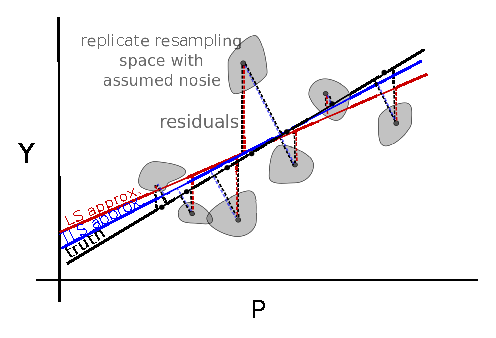
\includegraphics[width=.75\linewidth]{3/model_fit.eps}
% \caption{{\textbf Comparing residuals from regression methods.} Red lines show least squares and blue lines total least squares accounting for both independent and dependent variables. Grey areas around points illustrate zones of uncertainty probed by bootstrapping experimental replicate points.
% }
% \label{fig:modelFit}
% \end{figure}

\subsection{Network Inference}
\label{sec:netinf}
Networks arrange information regarding the interactions of constituent members in a manner prone to statistical analysis and often direct human consumption. In this context a node is generally in reference to a singular biomolecule, be it transcription factor, gene, intermediate gene product, protein, etc, which plays some role in the regulation of another such factor. Regulation comes about by a binding interaction of some sort dictated by the level of biology. This relational information is conveyed as a weight, the degree to which one factor influences another. As discussed previously, this weight can either convey up- or down- regulation.

Several approaches exist for this reverse engineering, ranging from an outdated assembly of one-to-one relationships to correlating patterns throughout expression assays and more.
Some inference methods return link existence with no confidence or weight, so called \emph{binary networks} (see \cref{sec:models}). In this and other scenarios, link weights can be estimated after link existence is establish. Such was the case after the creation of a null inferred network distribution, as in \textbf{Paper II}. Struggling to find a representative null distribution realistic enough to compare to and thus implement an FDR restriction, we refit inferred, shuffled network links using constrained least squares (CLS, \cref{eq:CLS} in the context of \cref{eq:Linearmap}) to improved their performance against measured links (detailed in the authors note in \cref{note}). 


\begin{equation}%\label{eqn:CLS}
\begin{aligned}\label{eq:CLS}
  \hat{\mA} = \arg \min_{\mA} & \sum \diag(\mDelta^T\mR \mDelta), \\
  \text{s.t.}\; & \mDelta = \mA \mY + \mP, \\
% \label{eqn:CLSPredErr} \\
  & \mR = \left( \hat{\mA}_{\textrm{init}} \Cov[\by] \hat{\mA}_{\textrm{init}}^{T} + \Cov[\bp]\right)^{-1},\\ %\label{eqn:CLSR} \\
  & \sign{\mA} = \sign{\hat{\mA}_{\textrm{reg}}}. \\
%   \label{eqn:CLSStructure}
\end{aligned}
\end{equation}
% \myequations{CLS}

This process is contained within the general balance fit error (BFE) algorithm in \textbf{Paper III}, wherein this optimization is iterated for balancing among input and output errors. This is done in order to minimize the overall error of the network reproducing the dataset in a leave-out manner, while still accounting for error inherent to the creation of the perturbation design matrix used in our linear model (\cref{eq:Linearmap}).

\subsection{Comparison to Null: Limiting Random Artifacts}
\label{sec:null}
The novelty and power of both \textbf{Paper II} and \textbf{Paper III} is drawn from a comparison to a null distribution of shuffled data and shuffled links, respectively. Networks inferred from shuffled data offer an estimate of how likely it is by chance to retrieve any given link otherwise constructing a bootstrap consensus network, and thereby restrict these links from inclusion. These links likely constitute false links and while returning more would do so at the cost of including more false links, increasing the \textbf{false discovery rate} (FDR) \citep{kall2007posterior}. In a similar way, testing how well shuffled GRN reproduce independent datasets allows testing of significance of how well your GRN inferred from real data can do the same. Furthermore, testing how well GRN reproduce training data compared to shuffled data. These null distributions are admittedly n{\"a}ive, but nevertheless have been shown to provide real improvement through their implementation in various pipelines here and elsewhere. Specifically, note such a null distribution is constructed from $10^5$ permuted label versions \cite{platig2016bipartite} in the COPD case study within the CONDOR publication for a similar comparison, lending significance to GWAS SNP data used to infer regulatory relationships between and among genes.